\chapter{Alternative geometry for the validation of buoyancy-driven flow}\label{appendixb}

In chapter \ref{chapter:validation} a vertical channel model is presented. Since velocity is given at the bottom of the channel, the model in chapter three is essentially a forced flow model. In various literature \cite{Wedin2001, Schillings2015}, this kind of setup is also used to simulate the buoyancy-driven flow, while the validation data comes from purely buoyancy-driven flow \cite{Boissonneau2000}. This is acceptable as long as the input velocity at the bottom comes from the experimental data.

However, an alternative setup can also be used to model a true buoyancy-driven flow without adding any velocity at the channel bottom. We set up geometry, as shown in figure \ref{naturalflowchannel}; the detailed geometry including the mesh is given in figure \ref{naturalchannel}.

\begin{figure}[H]
    \centering
    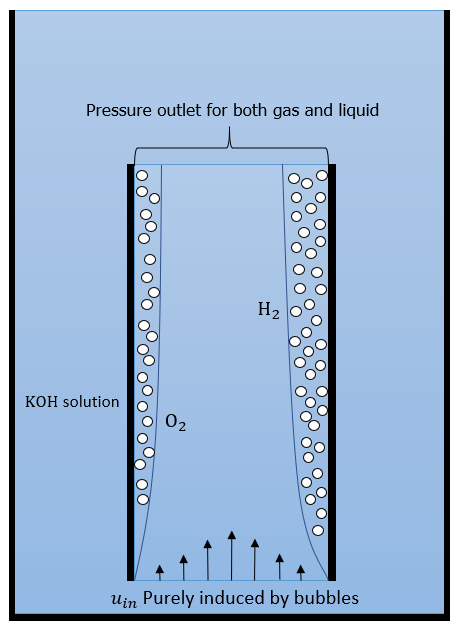
\includegraphics[scale=0.6]{naturalflowchannel.png}
    \caption{A sketch for the buoyancy driven flow}
    \label{naturalflowchannel}
\end{figure}

\begin{figure}[H]
    \centering
    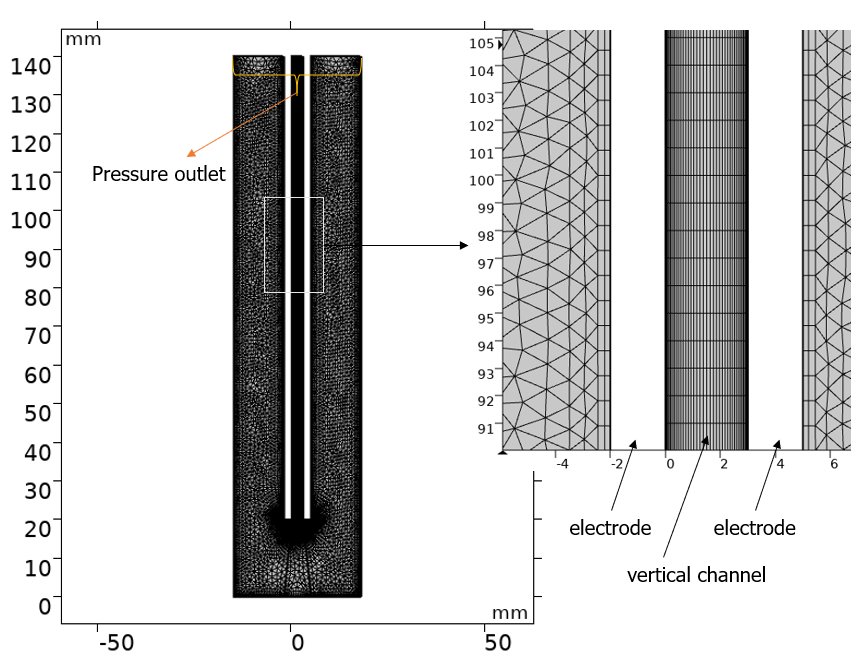
\includegraphics[scale=0.8]{naturalchannel.png}
    \caption{The geometry and the mesh for the buoyancy driven flow}
    \label{naturalchannel}
\end{figure}

\section*{Boundary conditions}

The boundary conditions are similar to that in chapter \ref{chapter:validation}, gases are evolved from both sides of the wall, and the top boundary is set as pressure outlet, only that no velocity is given at any boundary of the computation domain.

\section*{Results}

The velocity profiles at three different heights in the channel were compared with the same data with that in chapter \ref{chapter:validation}, and we can find that the simulation results without any inlet velocity also matches well with the experimental data.


\begin{figure}[H]
    \centering
    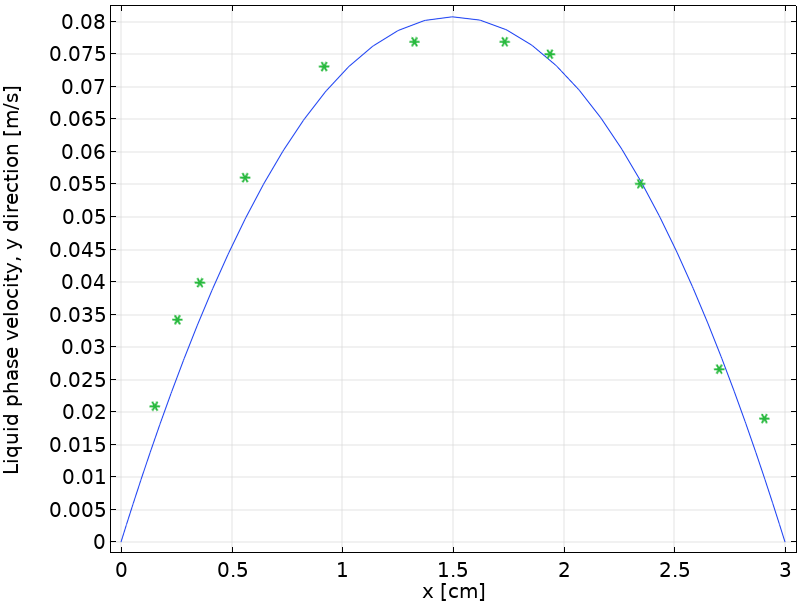
\includegraphics[width = 0.8\textwidth]{validation1.png}
    \caption{The velocity profile in the vertical channel at $y = 40 \, \mathrm{mm}$, $i_{av} = 1000 \, \mathrm{A/m^2}$}
    \label{validation1}
\end{figure}

\begin{figure}[H]
    \centering
    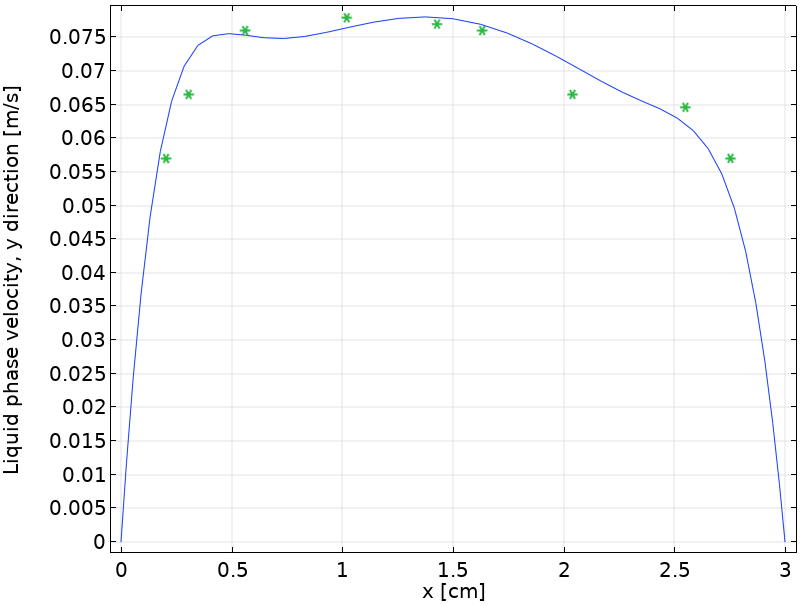
\includegraphics[width = 0.8\textwidth]{validation2.png}
    \caption{The velocity profile in the vertical channel at $y = 80 \, \mathrm{mm}$, $i_{av} = 1000 \, \mathrm{A/m^2}$}
    \label{validation2}
\end{figure}

\begin{figure}[H]
    \centering
    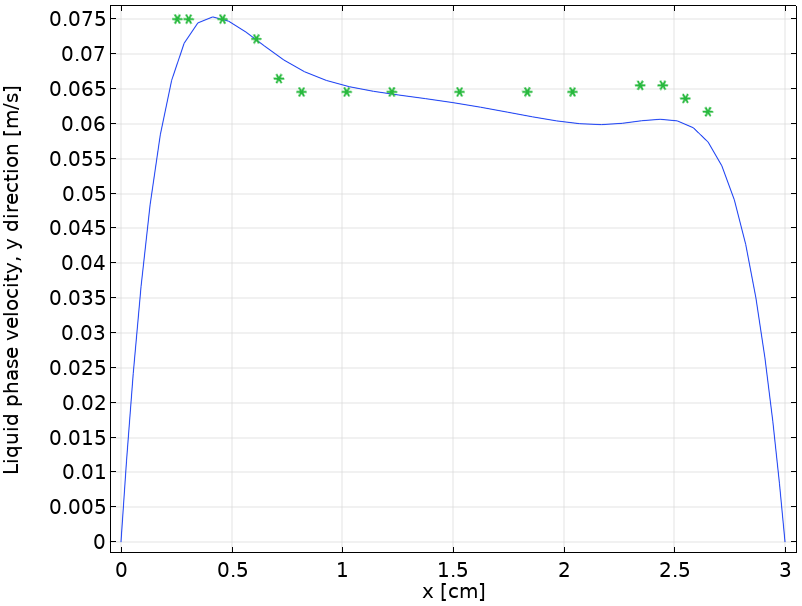
\includegraphics[width = 0.8\textwidth]{validation3.png}
    \caption{The velocity profile in the vertical channel at $y = 100 \, \mathrm{mm}$, $i_{av} = 1000 \, \mathrm{A/m^2}$}
    \label{validation3}
\end{figure}

% \section*{Transition to turbulence}

% Based on the description from Boissonneau et al.\cite{Boissonneau2000}, turbulence were indeed spotted in the vertical channel even under $i_{av} = 500 \, \mathrm{A/m^2}$. Moreover, both turbulent and laminar properties can exist at the same height because the turbulent intensity measured at the center of the channel is far less than in the bubbly plume. Here we try using the $k-\varepsilon$ model discussed in section \ref{turbulentmodel} to simulate the flow and focus on the top region of the channel where both velocity and volume fraction is higher. A velocity profile is shown in figure \ref{turbulentvelocityappendix}.

% In figure \ref{turbulentvelocityappendix} the velocity profile was fairly flat which is close to the profile in figure

% \begin{figure}[H]
%     \centering
%     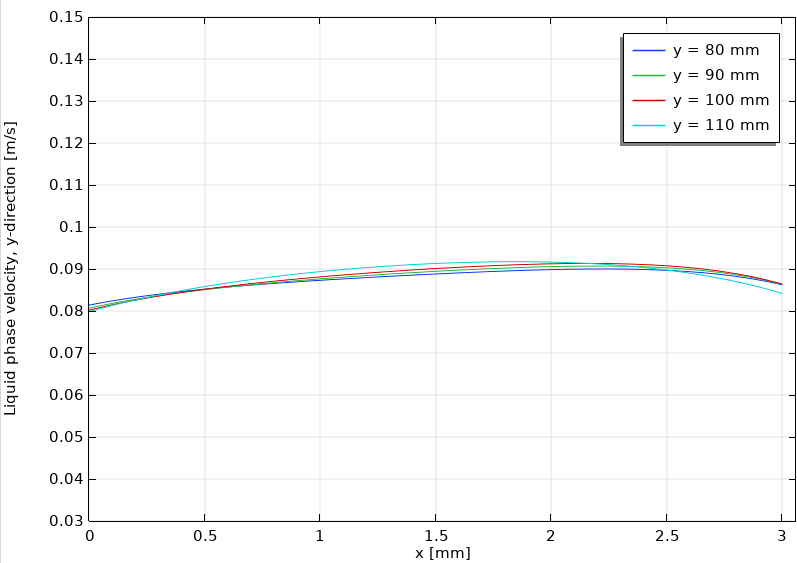
\includegraphics[width=\textwidth]{turbulentvelocityprofileappendix.png}
%     \caption{The velocity profile in the top region of the channel in $k-\varepsilon$ model, $i_{av} = 1000 \, \mathrm{A/m^2}$}
%     \label{turbulentvelocityappendix}
% \end{figure}